
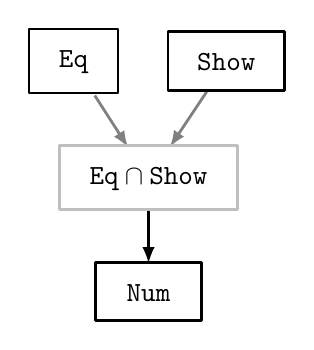
\begin{tikzpicture}[>=latex,line join=bevel,]
  \pgfsetlinewidth{1bp}
%%
\pgfsetcolor{black}
  % Edge: \texttt{Eq} -> \texttt{Eq} \cap \texttt{Show}
  \pgfsetcolor{gray}
  \draw [->] (23.665bp,82.077bp) .. controls (25.653bp,78.985bp) and (27.849bp,75.567bp)  .. (35.595bp,63.518bp);
  % Edge: \texttt{Eq} \cap \texttt{Show} -> \texttt{Num}
  \pgfsetcolor{black}
  \draw [->] (43bp,40.361bp) .. controls (43bp,37.7bp) and (43bp,34.793bp)  .. (43bp,21.685bp);
  % Edge: \texttt{Show} -> \texttt{Eq} \cap \texttt{Show}
  \pgfsetcolor{gray}
  \draw [->] (63.934bp,83.402bp) .. controls (61.612bp,79.917bp) and (58.948bp,75.922bp)  .. (50.753bp,63.63bp);
  % Node: \texttt{Show}
\begin{scope}
  \definecolor{strokecol}{rgb}{0.0,0.0,0.0};
  \pgfsetstrokecolor{strokecol}
  \draw (92bp,105bp) -- (50bp,105bp) -- (50bp,84bp) -- (92bp,84bp) -- cycle;
  \draw (71bp,94bp) node {$\texttt{Show}$};
\end{scope}
  % Node: \texttt{Num}
\begin{scope}
  \definecolor{strokecol}{rgb}{0.0,0.0,0.0};
  \pgfsetstrokecolor{strokecol}
  \draw (62bp,22bp) -- (24bp,22bp) -- (24bp,1bp) -- (62bp,1bp) -- cycle;
  \draw (43bp,11bp) node {$\texttt{Num}$};
\end{scope}
  % Node: \texttt{Eq}
\begin{scope}
  \definecolor{strokecol}{rgb}{0.0,0.0,0.0};
  \pgfsetstrokecolor{strokecol}
  \draw (32bp,106bp) -- (0bp,106bp) -- (0bp,83bp) -- (32bp,83bp) -- cycle;
  \draw (16bp,94bp) node {$\texttt{Eq}$};
\end{scope}
  % Node: \texttt{Eq} \cap \texttt{Show}
\begin{scope}
  \definecolor{strokecol}{rgb}{0.75,0.75,0.75};
  \pgfsetstrokecolor{strokecol}
  \draw (75bp,64bp) -- (11bp,64bp) -- (11bp,41bp) -- (75bp,41bp) -- cycle;
  \definecolor{strokecol}{rgb}{0.0,0.0,0.0};
  \pgfsetstrokecolor{strokecol}
  \draw (43bp,52bp) node {$\texttt{Eq} \cap \texttt{Show}$};
\end{scope}
%
\end{tikzpicture}

